\section{K. Hauser - Motion Planning for legged and humanoid robots \cite{Hauser2008}}
year: 2008
\subsection*{Summary}
The author defines the existence of different \textit{modes} $\sigma$ which belong to the same family $\Sigma$. The dimension of $\Sigma$, $dim(\Sigma)$, is lower than the dimension of the configuration space $Q$. All the modes of the same family are non-intersecting each other, meaning that if the robot is moving on a given trajectory $q$ which is on the mode $\sigma_1$ and wants to move to the mode $\sigma_2$ (of the same family $\Sigma$), it will have to go through another family $F$ which interesects the family $\Sigma$.
\subsection*{Key points / Takeaways}
\begin{itemize}
\item PRM = Probabilistic Road Map
\item MMPRM = Multi Modal Probabilistic Road Map
\item family = foliation
\item mode = leaves
\item In legged locomotion a \textbf{mode} $\sigma \in \Sigma$ is a fixed set of footfalls. So $\sigma$ stands for \textit{stance} and $Q_{\sigma}$ is the configuration space that can be reached by all the robots joints when the given stance $\sigma$ is fixed. In general a mode $\sigma$ defines a \textit{feasible space} $F_{\sigma}$ which is the set of configurations that satisfy the mode-specific constraints. Namely $F_{\sigma}$ is a subset of $Q$ (the configuration space of $q$), limited by the \textit{dimensionality reducing constraints} and by the \textit{volume reducing constraints}
\begin{figure}[h]
  \centering
  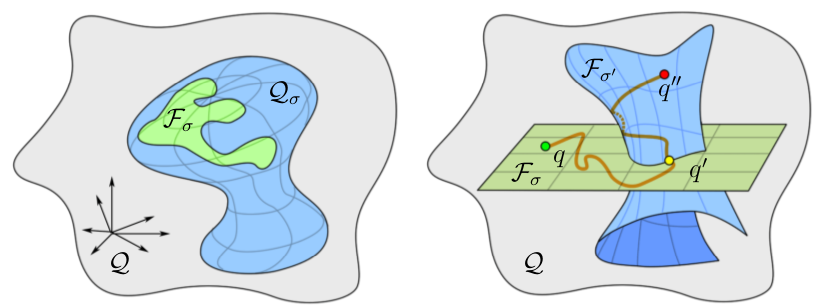
\includegraphics[width=120mm]{FamilyModes}
  \caption{Family modes}
  \label{OptimizationDiehl}
\end{figure}
\end{itemize}
\subsection*{Weak points}
\begin{itemize}
\item The author distinguishes between \textit{volume reducing constraints} and \textit{dimensionality reducing contraints}. And how can we classify the nonholonomic contraints then?
\end{itemize}

\subsection*{ideas}